% Created 2021-02-15 Mon 13:14
% Intended LaTeX compiler: pdflatex
\documentclass[english]{article}
\usepackage[T1, T2A]{fontenc}
\usepackage[lutf8]{luainputenc}
\usepackage[english, russian]{babel}
\usepackage{minted}
\usepackage{graphicx}
\usepackage{longtable}
\usepackage{hyperref}
\usepackage{xcolor}
\usepackage{natbib}
\usepackage{amssymb}
\usepackage{amsmath}
\usepackage{caption}
\usepackage{mathtools}
\usepackage{amsthm}
\usepackage{tikz}
\usepackage{grffile}
\usepackage{extarrows}
\usepackage{wrapfig}
\usepackage{rotating}
\usepackage{placeins}
\usepackage[normalem]{ulem}
\usepackage{amsmath}
\usepackage{textcomp}
\usepackage{capt-of}

\usepackage{geometry}
\geometry{a4paper,left=2.5cm,top=2cm,right=2.5cm,bottom=2cm,marginparsep=7pt, marginparwidth=.6in}

 \usepackage{hyperref}
 \hypersetup{
     colorlinks=true,
     linkcolor=blue,
     filecolor=orange,
     citecolor=black,      
     urlcolor=cyan,
     }

\usetikzlibrary{decorations.markings}
\usetikzlibrary{cd}
\usetikzlibrary{patterns}

\newcommand\addtag{\refstepcounter{equation}\tag{\theequation}}
\newcommand{\eqrefoffset}[1]{\addtocounter{equation}{-#1}(\arabic{equation}\addtocounter{equation}{#1})}


\newcommand{\R}{\mathbb{R}}
\renewcommand{\C}{\mathbb{C}}
\newcommand{\N}{\mathbb{N}}
\newcommand{\rank}{\text{rank}}
\newcommand{\const}{\text{const}}
\newcommand{\grad}{\text{grad}}

\theoremstyle{plain}
\newtheorem{axiom}{Аксиома}
\newtheorem{lemma}{Лемма}
\newtheorem{manuallemmainner}{Лемма}
\newenvironment{manuallemma}[1]{%
  \renewcommand\themanuallemmainner{#1}%
  \manuallemmainner
}{\endmanuallemmainner}

\theoremstyle{remark}
\newtheorem*{remark}{Примечание}
\newtheorem*{task}{Задача}
\newtheorem*{solution}{Решение}
\newtheorem{corollary}{Следствие}[theorem]
\newtheorem*{examp}{Пример}
\newtheorem*{observation}{Наблюдение}

\theoremstyle{definition}
\newtheorem{theorem}{Теорема}[section]
\newtheorem*{definition}{Определение}
\newtheorem*{symb}{Обозначение}
\newtheorem{manualtheoreminner}{Теорема}
\newenvironment{manualtheorem}[1]{%
  \renewcommand\themanualtheoreminner{#1}%
  \manualtheoreminner
}{\endmanualtheoreminner}
\captionsetup{justification=centering,margin=2cm}
\newenvironment{colored}[1]{\color{#1}}{}

\tikzset{->-/.style={decoration={
  markings,
  mark=at position .5 with {\arrow{>}}},postaction={decorate}}}
\makeatletter
\newcommand*{\relrelbarsep}{.386ex}
\newcommand*{\relrelbar}{%
  \mathrel{%
    \mathpalette\@relrelbar\relrelbarsep
  }%
}
\newcommand*{\@relrelbar}[2]{%
  \raise#2\hbox to 0pt{$\m@th#1\relbar$\hss}%
  \lower#2\hbox{$\m@th#1\relbar$}%
}
\providecommand*{\rightrightarrowsfill@}{%
  \arrowfill@\relrelbar\relrelbar\rightrightarrows
}
\providecommand*{\leftleftarrowsfill@}{%
  \arrowfill@\leftleftarrows\relrelbar\relrelbar
}
\providecommand*{\xrightrightarrows}[2][]{%
  \ext@arrow 0359\rightrightarrowsfill@{#1}{#2}%
}
\providecommand*{\xleftleftarrows}[2][]{%
  \ext@arrow 3095\leftleftarrowsfill@{#1}{#2}%
}
\makeatother
\author{Ilya Yaroshevskiy}
\date{\today}
\title{Лекция 2}
\hypersetup{
 pdfauthor={Ilya Yaroshevskiy},
 pdftitle={Лекция 2},
 pdfkeywords={},
 pdfsubject={},
 pdfcreator={Emacs 28.0.50 (Org mode )}, 
 pdflang={English}}
\begin{document}

\maketitle
\tableofcontents

\newcommand{\X}{\mathcal{X}}
\newcommand{\A}{\mathfrak{A}}

\section{Теореия меры}
\label{sec:org4f17b8c}
\subsection{Измеримые функции}
\label{sec:org9461656}
\begin{itemize}
\item \((X, \A, \mu)\)
\item \(f: X \to \overline{R}\) имзмерима
\item \(\forall a \in R\quad X(f < a) \in \A\)
\item \(\X_E\quad \sum \alpha_k \X_{E_k}\)
\end{itemize}
\begin{theorem}[характеризация измеримости функции с помощью ступенчатых]
\-
\begin{itemize}
\item \(f: X \to \overline{R}\)
\item \(f \ge 0\)
\item \(f\) --- измерима
\end{itemize}
\uline{Тогда} \(\exists f_n\) --- ступенчатая
\begin{enumerate}
\item \(0 \le f_1 \le f_2 \le \dots\)
\item \(\forall x f(x) = \lim_{n \to + \infty}f_n(x)\)
\end{enumerate}
\label{org4c71403}
\end{theorem}
\begin{proof}
\begin{center}
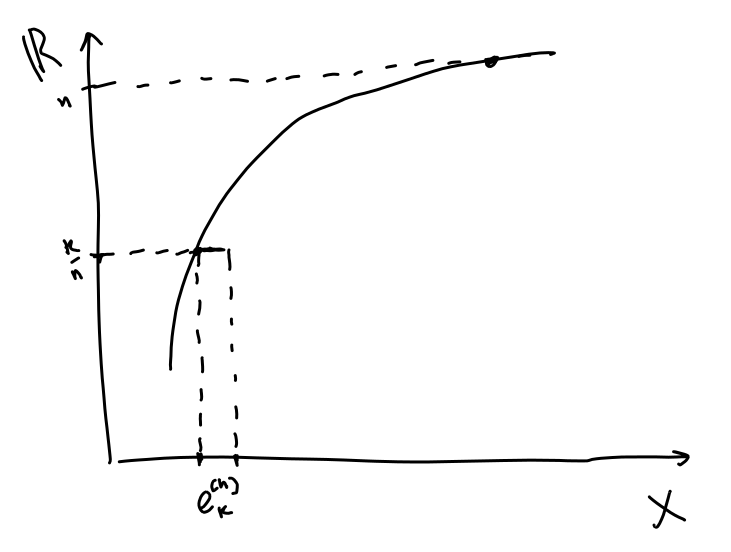
\includegraphics[scale=0.5]{2_1.png}
\end{center}
\[ e^{(n)}_k = X(\frac{k - 1}{n} \le f \le \frac{k}{n}) \quad k = 1,\dots,n^2 \]
\[ e^{(n)}_{n^2 + 1} = X(n \le f) \]
\[ g_n := \sum^{n + 1}_{k = 1} \frac{k - 1}{n} \X_{e^{(n)}_k} \]
\[ g_n \ge 0 \quad \lim_{n \to + \infty}g_n(x) = f(x) \]
\label{orgae76881}
\end{proof}
\begin{corollary}
\(f\) --- имзерима \\
\uline{Тогда} \(\exists f_n\) --- ступенчатая, \(f_n \xrightarrow{n \to + \infty}{} f\) всюду и \(|f_n| \le |f|\)
\label{org34e4768}
\end{corollary}
\begin{corollary}
\(f, g\) --- измеримы \\
\uline{Тогда} \(fg\) --- измемрима (\(0\cdot\infty=0\))
\label{orgf174c61}
\end{corollary}
\begin{proof}
\(f_n \to f\quad g_n \to g\), (\(f_n, g_n\)) --- ступеначтые \\
\(f_ng_n\) --- ступенчатая \(f_ng_n \to fg\)
\label{org5206326}
\end{proof}
\begin{corollary}
\(f, g\) --- измеримы \\
\uline{Тогда} \(f + g\) --- измерима
\label{org2df9d6e}
\end{corollary}
\begin{proof}
\(f_n \to f\quad g_n \to g\), (\(f_n, g_n\)) --- ступеначтые \\
\(f_n + g_n\) --- ступенчатая \(f_n + g_n \to f + g\) \\
\color{gray}Считаем что \(\forall x\), не может быть \(f(x) = \pm \infty,\ g(x) = \mp \infty\)
\label{org7597fe3}
\end{proof}

\begin{itemize}
\item \(A \subset X\)
\item \(A\) --- полная мера
\item \(\mu(X \setminus A) = 0\)
\end{itemize}
\begin{theorem}[об измеримости непрерывной на множестве полной меры]
\-
\begin{itemize}
\item \(f: E\to\R\)
\item \(E \subset \R^m\)
\item \(e \subset R\)
\item \(\lambda_me = 0\)
\item \(f\) --- непрерывна на \(E' = E \setminus e\)
\end{itemize}
\uline{Тогда} \(f\) --- измерима
\label{orged0fb03}
\end{theorem}
\begin{proof}
\(f\) --- измерима на \(E'\)  \\
\(E'(f < a)\) --- открыто в \(E'\) \\
\[ \left.\begin{array}{c} e(f < a) \subset e & \lambda_n \text{ --- полная}\end{array}\right\} \Rightarrow e(f < a)\text{ --- измерима в} E \]
\[ E(f < a) = E'(f < a) \cup e(f < a) \]
\label{orgcc285dd}
\end{proof}
\begin{examp}
\-
\begin{itemize}
\item \(E = \R\)
\item \(f = \X_{\text{Irr}}\)
\end{itemize}
\end{examp}
\begin{corollary}
\-
\begin{itemize}
\item \((X, \A, \mu)\)
\item \(f: E\to\R\)
\item \(e \subset E \subset X\)
\item \(E' = E \setminus e\)
\item \(f\) --- измерима на \(E'\)
\end{itemize}
\uline{Тогда} модно так переопределить \(f\) на множестве \(e\), что полученая функция \(\tilde{f}\) будет измерима на \(E\)
\end{corollary}
\begin{proof}
Пусть:
\[ \tilde{f} = \left\{\begin{array}{ll}f(x) & , x \in E \\ \const & ,x \in e \end{array} \]
\[ E(\tilde{f} < a) = E'(\tilde{f} < a)\cup e(\tilde{f} < a) \]
\end{proof}
\begin{corollary}
\(f: \langle a, b \rangle \to \R\) --- монотонна \\
\uline{Тогда} \(f\) --- измерима
\end{corollary}
\begin{proof}
\(f\) --- непрерывна на \(\langle a, b \rangle\) за исключением возможно счетного числа точек
\end{proof}
\subsection{Сходимость почти везде и по мере}
\label{sec:org3614c4e}
\begin{defintion}
\begin{itemize}
\item \((X, \A, \mu)\)
\item \(E \in \A\)
\item \(W(x)\) --- высказывание (\(x\in X\))
\end{itemize}
\(W(x)\) --- верное при почти всех \(x \in E\)
\begin{description}
\item[{=}] почти всюду на \(E\)
\item[{=}] почти везде на \(E\)
\end{description}
\(\exists e \subset E\quad \mu e= 0\quad W(x)\) --- истино при \(x \in E \setminus e\)
\end{defintion}
\begin{examp}
\(x = \R\), \(x\) --- иррационально
\end{examp}
\begin{examp}
\(f_n(x) \xrightarrow{}{n \to + \infty} f(x)\) при почти всех \(x \in E\) \\
\(\exists e, \mu e = 0\), при \(x\in E \setminus e\quad f_n(x) \xrightarrow[n \to + \infty]{}f(x)\) \\
\end{examp}
\begin{remark}
Свойства: \\
\begin{enumerate}
\item \(\mu\) --- полная \(f_n,f: X \to \overline{\R}\) \\
\(\left.\begin{array}{l}
   f_n(x) \to f(x) \text{ почти везде на }X \\
   f_n \text{ --- измерима}
   \end{array}\right|\) Тогда \(f\) --- измерима
\begin{proof}
\(f_n \to f\) на \(X'\), где \(e = X \setminus X', \mu e = 0\) \\
\(f\) --- измерима на \(X'\) \\
\(\mu\) --- полная \(\Rightarrow\) \(f\) --- измерима на \(X\) \\
\[ X(f < a) = \underset{\text{изм.}}{X'(f < a)}\cup e(f < a) \]
\end{proof}
\item В условии п. 1 \\
Можно переопределить \(f\) на \(e\). Получится \(\hat{f}\) \\
\(f_n(x) \to \hat{f}(x)\) почти везде \\
\(\hat{f}\) --- измкрима
\begin{definition}
\(f = g\) почти везде \\
Будем говорить что \(f\) и \(g\) эквивалентны
\end{definition}

\item Пусть \(\forall n\ W_n(x)\) --- истинно при почти всех \(x\) \\
\uline{Тогда} утверждение \("\) \(\forall n\ W_n(x)\) --- истинно \("\) --- верно при почти всех \(x\) \\
Это высказывание верно при \[ x \in X \setminus (\bigcup_{i = 1}^{+ \infty} e_i)\quad\mu(\bigcup e_i) = 0 \]
\end{enumerate}
\end{remark}
\begin{defintion}
\-
\begin{itemize}
\item \(f_n, f : X \to \overline{\R}\) --- почти везде конечные \\
\item \(f_n\) сходится к \(f\) по мере
\item \(f_n \xRightarrow[\mu]{} f: \forall \varepsilon > 0\ \mu X(|f_n - f| \ge \varepsilon) \xrightarrow[n \to + \infty]{} 0\)
\end{itemize}
\end{defintion}
\begin{remark}
\(f_n\) и \(f\) можно изменить на множестве меры 0 \\
Т.е. предел не задан однозначно
\end{remark}
\begin{examp}
\-
\begin{center}
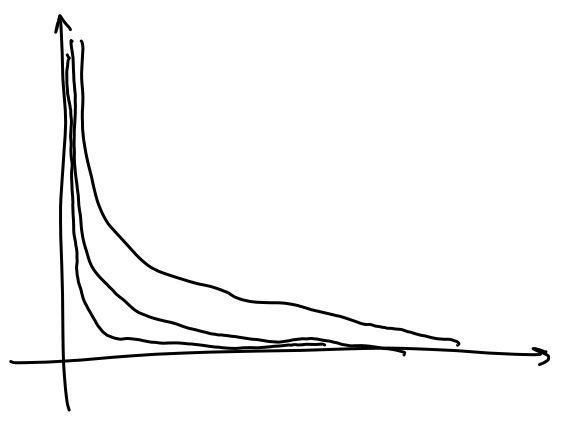
\includegraphics[scale=0.3]{2_2.png}
\end{center}
\(f_n(x) = \frac{1}{nx}, x > 0\) \\
\(X \ \R_+\ \lambda\) \\
\(f_n \to f\) всюду на \((0, + \infty)\) \\
\(f_n \xRightarrow[\lambda]{} f\)
\end{examp}
\begin{examp}
\-
\begin{center}
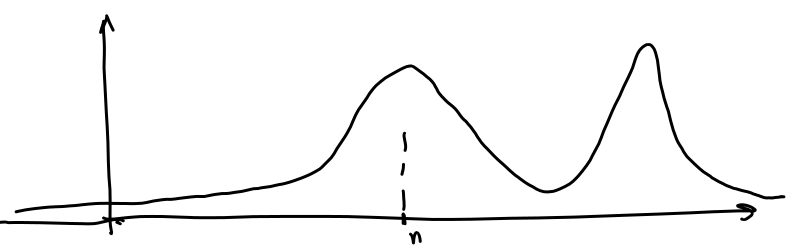
\includegraphics[scale=0.3]{2_3.png}
\end{center}
\(f_n(x) := e^{-(n - x)^2}\ x \in \R\) \\
\(f_n(x) \to 0\) при всех \(x\) \\
\(f_n(x) \rightarrow 0\) \\
\[ \mu (\R(e^{-(n - x)^2} \ge \varepsilon)) = \const \not\to 0 \]
, при \(0 < \varepsilon < 1\)
\end{examp}
\begin{examp}
\(n = 2^k + e, 0 \le e < 2^k\) \\
\(X = [0, 1]\ \lambda\) \\
\(f_n(x) := \X_{[\frac{e}{2^k}, \frac{e + 1}{2^k}]}\) \\
\(\lim f_n(x)\) --- не существует ни при каких \(x\) \\
\[ \lambda X(f_n > \varepsilon) = \frac{1}{2^k} \xrightarrow[n \to + \infty]{} 0 \]
\[ f_n \xRightarrow[\lambda]{} 0 \]
\end{examp}
\begin{theorem}[Лебега]
\-
\begin{itemize}
\item \((X, \A, \mu)\)
\item \(f_n, f\) --- измеримые, почти везде конечные
\item \(f_n \to f\) почти везде
\item \(\mu X\) --- конечна
\end{itemize}
\uline{Тогда} \(f_n \xRightarrow[\mu]{} f\)
\end{theorem}
\begin{proof}
Переопределим \(f_n, f\) на множестве меры 0, чтобы сходимость была всюду
\uline{Частный случай}: \(\forall x\) последовательность \(f_n(x)\) монотонно убывает к 0(т.е. \(f < 0\))
\[ \left.\begin{array}{cc}X(|f_n| \ge \varepsilon) = X(f_n \ge \varepsilon) \supset X(f_{n + 1} \ge \varepsilon) \\ \bigcap X(f_n \ge \varepsilon) = \emptyset \end{array}\right\} \Rightarrow \text{Теорема о непрерывность меры сверху}\]
\uline{Общий случай}: \(f_n \to f\)
\[ \varphi_n(x) = \sup_{k \ge n}|f_k(x) - f(x)| \]
Тогда \(\varphi_n \to 0\), монотонна
\[ X(|f_n - f| \ge \varepsilon) \subset X(\varphi_n \ge \varepsilon) \]
\[ \mu X(|f_n - f| \ge \varepsilon) \le \mu X(\varphi_n \ge \varepsilon) \to 0 \]
\end{proof}
\begin{theorem}[Рисс]
\-
\begin{itemize}
\item \((X, \A, \mu)\)
\item \(f_n, f\) --- измеримы почти везде, конечны
\item \(f_n \xRightarrow[\mu]{} f\)
\end{itemize}
\uline{Тогда} \(\exists n_k f_{n_k} \to f\) почти везде
\end{theorem}
\begin{proof}
\(\forall k\ \mu X(|f_n - f| \ge \frac{1}{k}) \to 0\) \\
\(\exists n_k\): при \(n > n_k\ \mu X(|f_n - f| \ge \frac{1}{k}) < \frac{1}{2^k}\) \\
можно считать: \(n_1 < n_2 < n_3\) \\
Проверим \(f_{n_k} \to f\) почти везде
\[ E_k := \bigcup_{i = k}^{+ \infty} X(|f_{n_i} - f| \ge \frac{1}{i})\quad E = \bigcap E_i \]
\[ E_k \supset E_{k + 1}\quad \mu E_k \le \sum_{i = k}^{+ \infty}\mu X(|f_{n_i} - f| \ge \frac{1}{i}) < \sum_{i = k}^{+ \infty}\frac{1}{2^i} \le \frac{2}{2^k} \to 0 \]
\[ \mu E_k \to \mu E \Rightarrow \mu E = 0 \]
При \(x \not\in E\ f_{n_k} \to f\) \\
\[ x\not\in E\ \exists N\ x\not\in E_k$ при $k > N \quad |f_{n_k}(x) - f(x)| < \frac{1}{k} \]
, т.е. \(f_{n_k}(x) \to f(x)\)
\end{proof}
\begin{corollary}
\-
\begin{itemize}
\item \(f_n \xRightarrow[\mu]{} f\)
\item \(|f_n| \le g\) почти везде
\end{itemize}
\uline{Тогда} \(|f| \le g\) почти везде
\end{corollary}
\begin{proof}
\(\exists n_k:\ f_{n_k} \to f\) почти везде
\end{proof}
\begin{theorem}[Егорова]
\-
\begin{itemize}
\item \(\mu X < + \infty\)
\item \(f_n, f\) --- почти везде конечны, измеримы
\item \(f_n \to f\) почти везде
\end{itemize}
\uline{Тогда}  \(\forall \varepsilon > 0\ \exists e \subset X,\ \mu e < \varepsilon\quad f_n \rightrightarrows f\) на \(X \setminus e\)
\end{theorem}
\xymatrix@1{A\ar[r]^>>{+}&B}

\section{Интеграл}
\label{sec:orgffe8cf8}
\((X, \A, \mu)\)
\begin{definition}
\label{def_int_1}
\(f = \sum \alpha_k \X_{E_k}\quad\begin{array}{c} E_k\text{ --- дополнительное разбиение} \\ \alpha_k \ge 0 \end{array}\) \\
\[ \int_X f d\mu = \sum \alpha_k \mu E_k \]
, считаем \(0\cdot + \infty = 0\)
\end{definition}
\begin{remark}
Свойства:
\begin{enumerate}
\item Не зависит от представления \(f\) в виде сумме \\
\[ f = \sum \alpha_k \X_{E_k} = \sum \alpha'_k\X_{E'_k} = \sum_{k,j}\alpha_k \X_{E_k\cap E'_j} \]
\[ \int f = \sum \alpha_k \mu E_k \]
\item \(f \le g\quad\int f \le \int g\), \(f, g\) --- ст.
\end{enumerate}
\end{remark}
\begin{definition}
\label{def_int_2}
\(f \ge 0\) --- измерима \\
\[ \int_X f d\mu := \sup_{\substack{g\text{ --- ступ.} \\ 0 \le g \le f}} \int g d\mu \]
\end{definition}
\begin{remark}
Свойства:
\begin{enumerate}
\item Если \(f\) --- ступенчатая то \hyperref[def_int_1]{Опр. 2} = \hyperref[def_int_2]{Опр. 1}
\item \(0 \le \int f \le + \infty\)
\item \(g \le f\), \(f\) --- измерима, \(g\) --- ступенчатая \(\Rightarrow\) \(\int_X g \le \int_X f\)
\end{enumerate}
\end{remark}
\begin{definition}
\-
\begin{itemize}
\item \(f\) --- измерима
\item \(\int_X f^+\) или \(\int_x f^-\) конечный
\end{itemize}
\uline{Тогда} \[ \int_X f d\mu = \int_X f^+ d\mu - \int_X f^- d\mu \]
\end{definition}
\begin{theorem}[Тонедди]
\-
\begin{itemize}
\item \(f: \R^{m + n} \to \overline{\R}\)
\item \(f \ge 0\) --- измерима
\item \(E \subset \R^{m + n}\)
\end{itemize}
\begin{symb}
\(\forall x \in \R^m\quad E_x = \{ y\in\R^n : (x, y) \in E\}\)
\end{symb}
\uline{Тогда}
\begin{center}
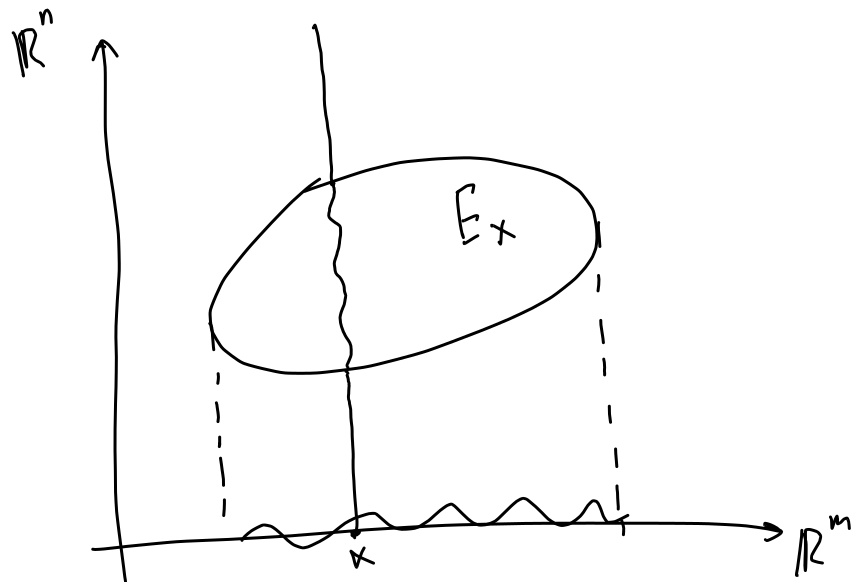
\includegraphics[scale=0.3]{2_4.png}
\end{center}
\begin{enumerate}
\item при почти всех \(x \in \R^m\) функция \(y\mapsto f(x, y)\) --- измерима на \(\R^n\)
\item функция \[ x \mapsto \int_{E_k} f(x, y) d\lambda_n(y) \ge 0 \]
\item \[ \int_E f(x, y) d\mu = \int_{\R^m}\left(\int_{E_x} f(x, y d\lambda_n(y))\right)d\lambda_m(x) \]
\end{enumerate}
\end{theorem}
\end{document}
